\chapter{Spatial Transformations for the Computations of the Log-composition: $SE(2)$ and $\text{Diff}(\Omega)$}\label{ch:spatial_transformations}


\begin{flushright}
	\emph{Every working mathematician knows that if one does not control oneself (best of all by examples), then after some ten pages half of all the signs in formulae will be wrong and twos will find their way from denominators into numerators. \\ -V.I. Arnold}
\end{flushright}

\noindent
In the previous chapter we have introduced some essential mathematical tools for the numerical computation of the log-composition. Each of the theoretical elements depends strongly on the transformations considered, and in this chapter we will see how they can be applied for the transformations belonging to $SE(2)$ and $\text{Diff}(\Omega)$.
%\begin{enumerate}
%	\item[$SE(2)$ -] The group of rigid body transformation of the plane (any combination of bi-dimensional rotations and translations) is a good playground to test the numerical methods for the computation of the log-composition introduced so far, since results can be compared with a ground truth.
%	\item[$\text{Diff}(\Omega)$ -] The group of diffeomorphisms over $\Omega$, indcated with $\text{Diff}(\Omega)$ is defined over the wide set of all of the differentiable and invertible functions. For our applications we will restrict the set to the diffeomorphisms that can be parametrized by stationary velocity fields or SVF. This infinite dimensional vector space is the second algebra utilized to test the numerical methods for the computation of the log-composition. In this case we do not know any closed form, but considering an \lq\lq improper norm\rq\rq~ in the space of deformations it is possible to compare SVF and assess the quality of the results.
%\end{enumerate}


\section{The Lie Group of Rigid Body Transformations}\label{se:rigid_body_transformations}
% group
Each element of the group of rigid body transformation (or euclidean group) $SE(2)$ can be computed as the consecutive application of a rotation and a translation applied to any point $(x,y)^T$ of the plane:
\begin{align*}
\left (  
\begin{array} {c }
X \\
Y
\end{array}
\right )  
= 
R(\theta)
\left (  
\begin{array} {c }
x \\
y
\end{array}
\right ) 
+
t
=
\left (
\begin{array} {c c }
\cos(\theta) & - \sin(\theta) \\
\sin(\theta) & \cos(\theta) 
\end{array}
\right )
\left (  
\begin{array} {c }
x \\
y
\end{array}
\right ) 
+
\left (  
\begin{array} {c }
t^x \\
t^y
\end{array}
\right ) 
\end{align*}
where the rotation matrix indicated with $R(\theta)$ belongs to the special orthogonal group $SO(2)$ and the translation $t$ is a vector of the plane.\\
We can represent the elements of $SE(2)$ in two different form: as ternary vector (restricted form) 
\begin{align*}
SE(2)^{v} 
:=
\{ (\theta, t^x, t^y) \mid \theta \in [0, 2\pi),   t^x, t^y \in\mathbf{R}^2  \}
\end{align*}
or with matrices (matrix form)
\begin{align*}
SE(2) 
:= 
\left \{
\left (
\begin{array} {c c }
R(\theta) & t \\
0 & 1 
\end{array}
\right )
=
\left (
\begin{array} {c c c }
\cos(\theta) & - \sin(\theta)& t^{x} \\
\sin(\theta) & \cos(\theta) & t^{y}\\
0 & 0 &  1
\end{array}
\right )
\mid
\theta \in  [0, 2\pi), (t^x, t^y) \in\mathbf{R}^2
\right \}
\end{align*}
The group $SE(2)$ it is a manifold with a differentiable structure compatible with the operation of composition, whose Lie algebra is given in matrix form by
\begin{align*}
\mathfrak{se}(2) := 
\left \{
\left (
\begin{array} {c c }
dR(\theta) & dt \\
0 & 0
\end{array}
\right )
=
\left (
\begin{array} {c c c }
0 & -\theta &  dt^{x} \\
\theta & 0 & dt^{y} \\
0& 0 & 0
\end{array}
\right )
\mid
\theta \in  [0, 2\pi), (dt^x, dt^y) \in\mathbf{R}^2
\right \}
\end{align*}
and it is indicated with $\mathfrak{se}(2)^{v}$ in its restricted form.

Given $r$, element of $SE(2)$ with $\theta\neq 0$, its image with the Lie group logarithm is
\begin{align*}
\log(r)
&=
\sum_{k=1}^{\infty} (-1)^{k+1}~\frac{(r - I)^k}{k}
=
\left (
\begin{array} {c c }
dR(\theta) & L(\theta)t \\
0 & 1 
\end{array}
\right )
\\
&=
\left (
\begin{array} {c c c}
0   & - \theta& \frac{\theta}{2} (\frac{\sin(\theta)}{1-\cos(\theta)} t^x + t^y )\\
\theta & 0     & \frac{\theta}{2} (- t^x + \frac{\sin(\theta)}{1-\cos(\theta)} t^y )\\
0 & 0 &  0
\end{array}
\right )
\end{align*}
where 
\begin{align*}
dR(\theta) = 
\left (
\begin{array} {c c }
0 & -\theta \\
\theta & 0 
\end{array}
\right )
\qquad \qquad 
L(\theta) = 
\frac{\theta}{2}
\left (
\begin{array} {c c }
\frac{\sin(\theta)}{1-\cos(\theta)} & 1 \\
-1 & \frac{\sin(\theta)}{1-\cos(\theta)}
\end{array}
\right )
\end{align*}
On the way back, the exponential of $dr \in \mathfrak{se}(2)$ is given by:
\begin{align*}
\exp(dr)
&=
\sum_{k=1}^{\infty} \frac{dr^{k}}{k!}
=
\left (
\begin{array} {c c }
R(\theta) & L(\theta)^{-1}dt \\
0 & 1 
\end{array}
\right )
\\
&=
\left (
\begin{array} {c c c}
\cos(\theta)   & - \sin(\theta)& \frac{1}{\theta} (\sin(\theta)dt^x - (1-\cos(\theta)) dt^y )\\
\sin(\theta) & \cos(\theta)     & \frac{1}{\theta} (- (1-\cos(\theta))dt^x + \sin(\theta) dt^y )\\
0 & 0 &  1
\end{array}
\right )
\end{align*}
where
\begin{align*}
L(\theta)^{-1} = 
\frac{1}{\theta}
\left (
\begin{array} {c c }
\sin(\theta) & -(1-\cos(\theta)) \\
(1-\cos(\theta)) & \sin(\theta)
\end{array}
\right )
\end{align*}
When $\theta$ is zero, $R(\theta)$ and $dR(\theta)$ coincide with the identity, and the transformation results in a translation. For proof and further details see for example \cite{gallier2011geometric} \cite{hall2015lie}.

At this point it is important to notice that: 
\begin{enumerate}
	%infinite series 
	\item The infinite series of matrices  do not raises any theoretical issues, since the sum is defined in the group as subset of a bigger algebra that contains both the Lie group and the Lie algebra. It appears to be the natural way to move back and forth from the group to the algebra. A second door to passing from one structure to the other, when the rotation $\theta$ is small is provided by the following approximations:
	\begin{align}\label{eq:small_rotation_matrices_approx}
	\exp(r) \simeq I + r
	\qquad 
	\log(dr) \simeq dr - I
	\end{align}
	In fact for small $\theta$, $\sin(\theta) \simeq \theta$, $\cos(\theta) \simeq 0 $ and $ L(\theta) \simeq I$.
   %
	\begin{figure}[!ht]
		\centering
		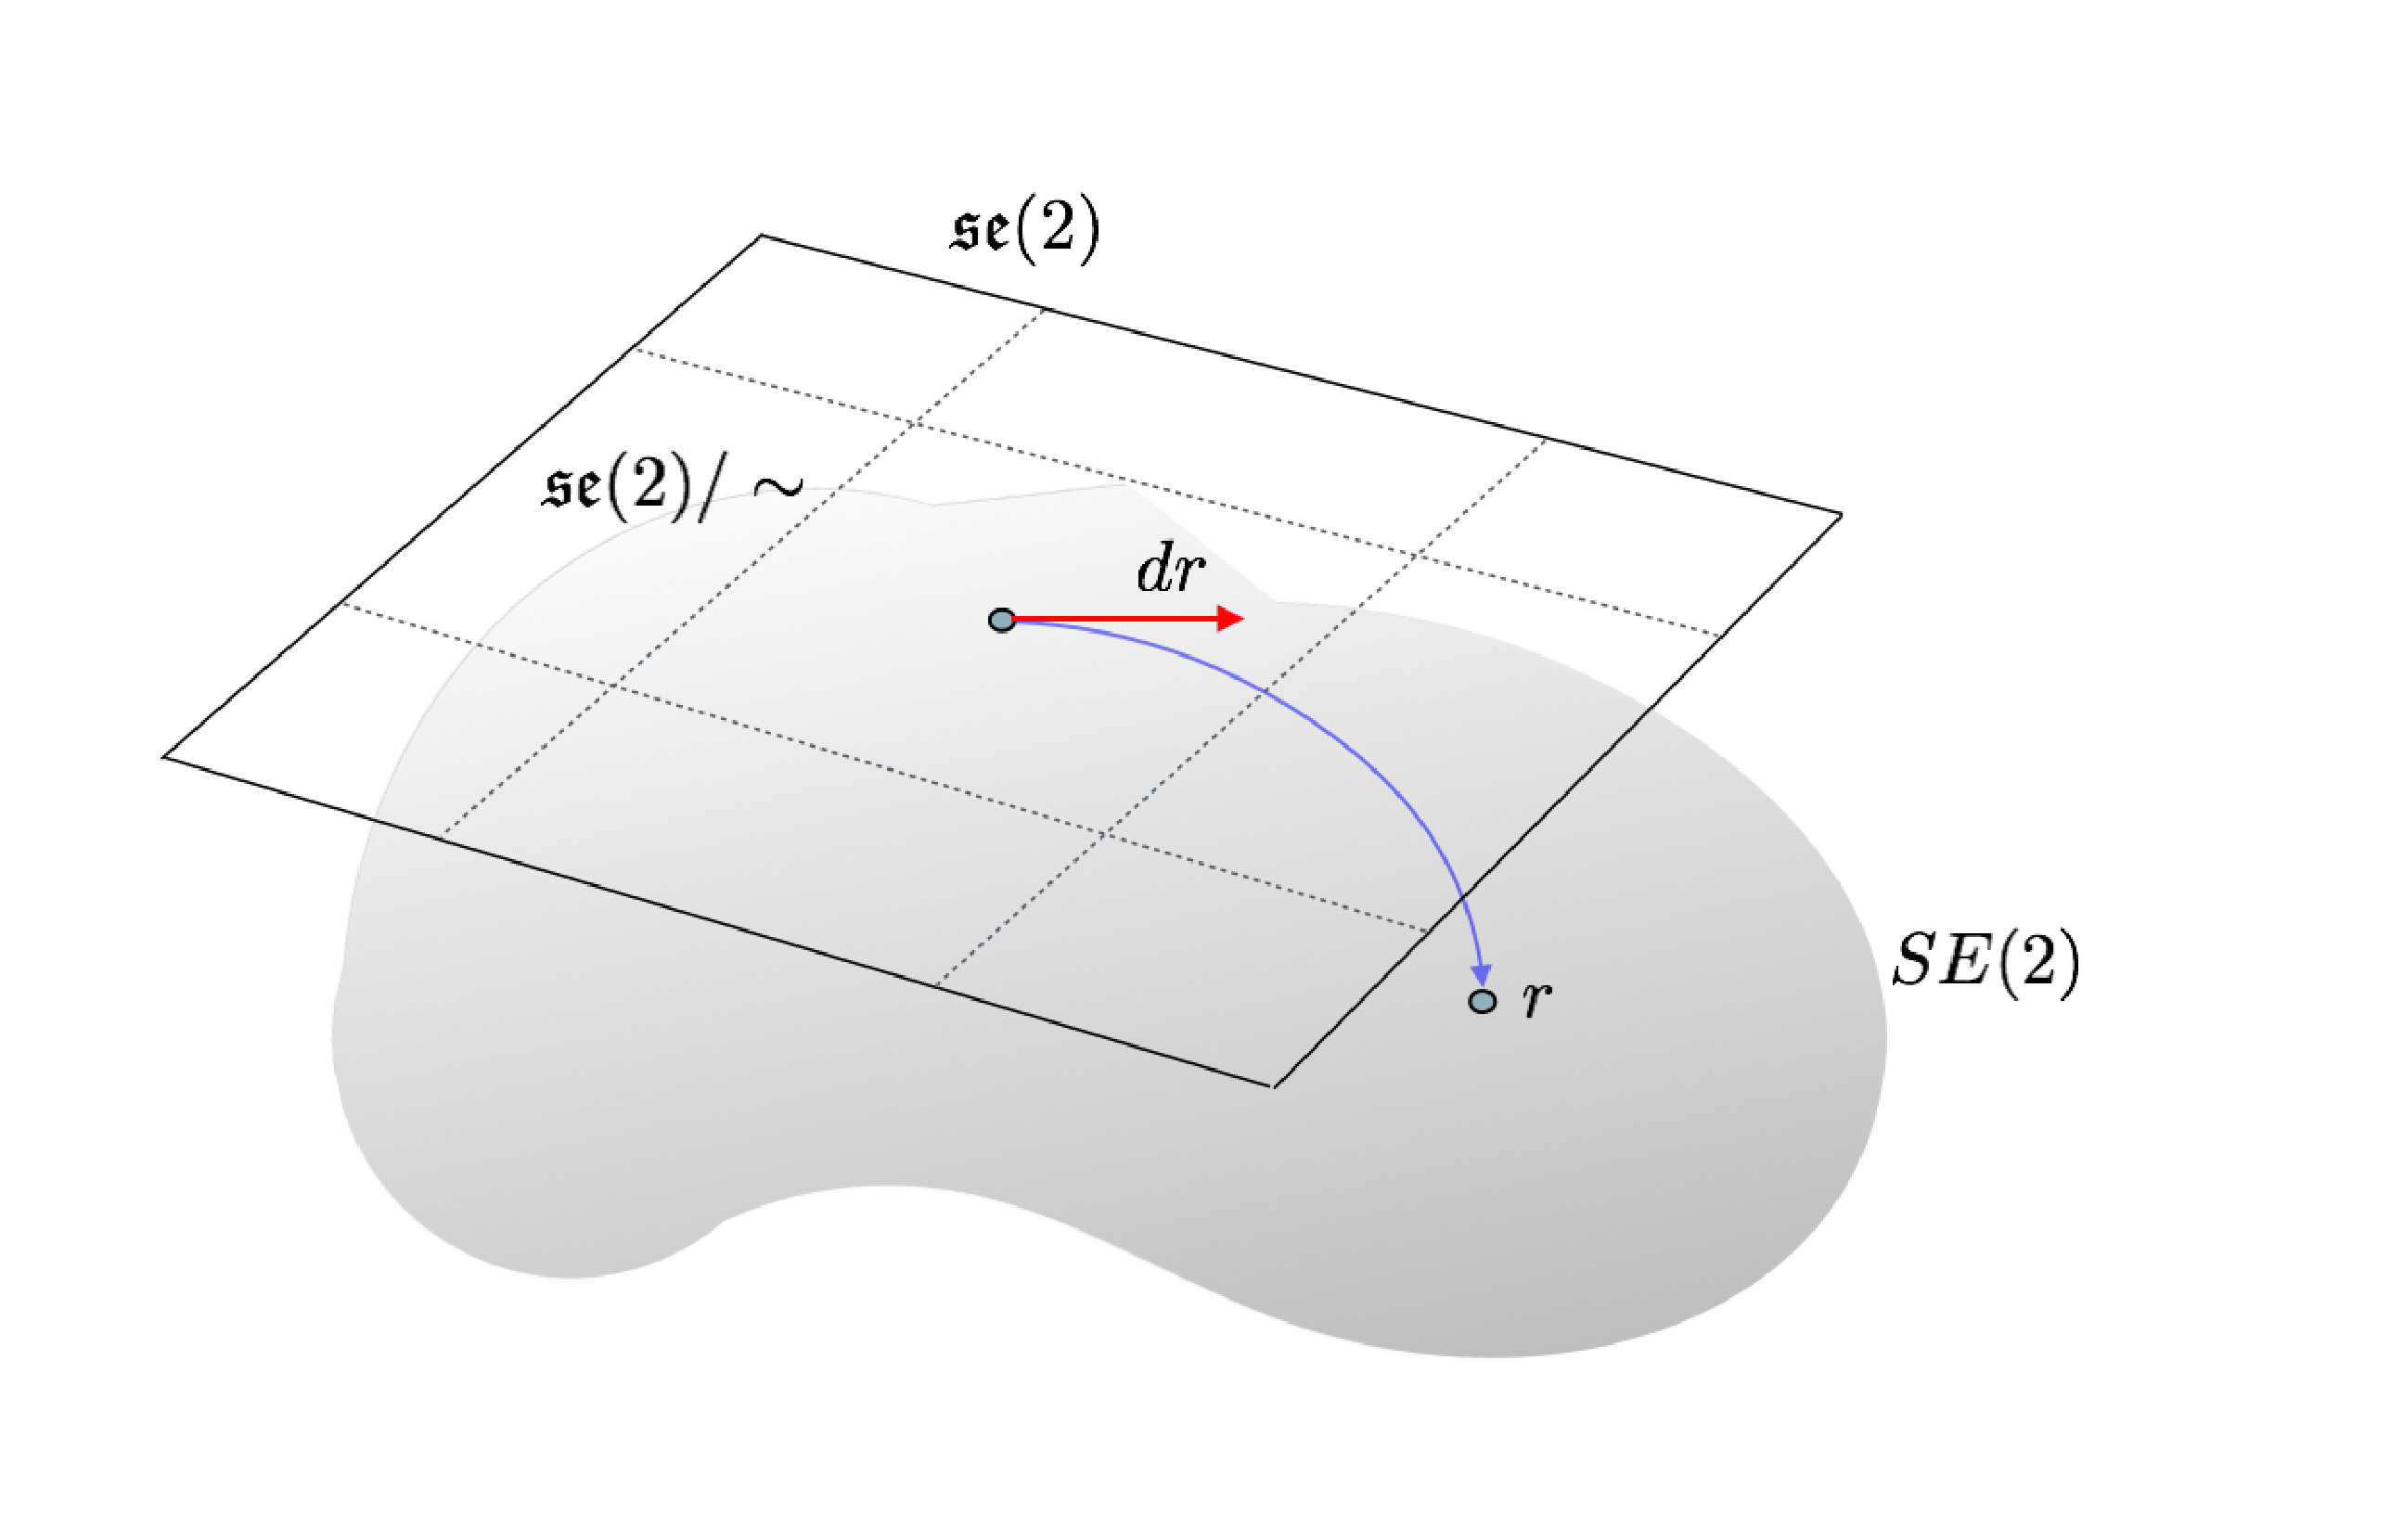
\includegraphics[scale=0.35]{figures/exp_se2.pdf}
		\caption{The Lie algebra $\mathfrak{se}(2)/\sim$ defined as the quotient of the Lie algebra $\mathfrak{se}(2)$ over the equivalence relation $\sim$ is in bijective correspondence with $SE(2)$.}
		\label{fig:exp_se2}
	\end{figure}
	% restriction of the domain.
	\item The map $\exp$ is not well defined as bijection over its whole domain $\mathfrak{se}(2)$. Given two elements $(\theta_0, dt^{x}_0, dt^{y}_0)$ and $(\theta_1, dt^{x}_1, dt^{y}_1)$, they have the same image with $\exp$ function if the two following conditions are both satisfied:
	\begin{enumerate}
		\item[i)] Exists an integer $k$ such that $\theta_0 = \theta_1 + 2k\pi$.
		\item[ii)] the translation $(dt^{x}_0, dt^{y}_0)$ coincides with $(dt^{x}_1, dt^{y}_1)$ up to a factor $\frac{\theta_0}{\theta_1}$, where the angles are considered modulo $2\pi$.
	\end{enumerate}
	To have a bijective correspondence the domain of $\exp$ has to be restricted to a space where if $\exp(\theta_0, dt^{x}_0,dt^{y}_0) = \exp(\theta_1, dt^{x}_1, dt^{y}_1)$ implies  $(\theta_0, dt^{x}_0, dt^{y}_0) = (\theta_1, dt^{x}_1, dt^{y}_1)$.
	It can be easy to prove that the sought space is the quotient of $\mathfrak{se}(2)$ over the equivalence relation $\sim$, defined as 
	\begin{align*}
		(\theta_0, dt^{x}_0, dt^{y}_0 & ) \sim (\theta_1, dt^{x}_1, dt^{y}_1)
		\\
		&\iff_{\text{(by definition)}}
		\\
		\exists k\in\mathbb{Z} \mid \theta_0 = \theta_1 + 2k\pi 
		&~\text{ and }~
		(dt^{x}_0, dt^{y}_0) = \frac{\theta_0}{\theta_1}(dt^{x}_1, dt^{y}_1)
	\end{align*}
	The new algebra defined by the set of equivalence classes of this relation is indicated - with the standard convention, see \cite{artin2011algebra} - with $\mathfrak{se}(2)/\sim$. With this restriction of the domain, the function $\exp$ is a bijection having $\log$ as its inverse.
	What said so far can be summarize in the following commutative diagram:
	
	\[
	\begindc{\commdiag}[40]
	\obj(55,15)[u]{$\mathfrak{se}(2)/\sim $}
	
	%rightside
	\obj(35,30)[se]{$\mathfrak{se}(2)$}
	\obj(35,0)[SE]{$SE(2)$}
	
	% oblique right
	\mor{se}{u}{$\pi$} [\atright,\surjectivearrow]
	\mor{u}{SE}{$\exp$}
	% vertical
	\mor{SE}{se}{$\log$} 
	
	\enddc
	\]

	and with the schematic figure \ref{fig:exp_se2}.
	
\end{enumerate}

% % % % % % % % % % % % % % % % % %
% % % % % % % % % % % % % % % % % % %
\subsection{Computations of Log-composition in $\mathfrak{se}(2)$}
The log-composition of two elements $dr_0 = (\theta_0, dt^{x}_0, dt^{y}_0)$ ans $dr_1 = (\theta_1, dt^{x}_1, dt^{y}_1)$ of $ \mathfrak{se}(2)/\sim$ results
\begin{align}\label{eq:log_composition_se2_closed_form}
& dr_0 \oplus dr_1 =  \log(\exp(dr_0)\circ \exp(dr_1)) 
\end{align}
The approximations of the log-composition using truncated BCH formulas are straightforward:
\begin{align*}
dr_0 \oplus dr_1 &\simeq  BCH^{0}(dr_0,dr_1 ) := dr_0 + dr_1  \\
dr_0 \oplus dr_1 &\simeq BCH^{1}(dr_0,dr_1 ) :=  dr_0 + dr_1 + \frac{1}{2}[dr_0, dr_1] \\
dr_0 \oplus dr_1 &\simeq BCH^{3/2}(dr_{0}, dr_{1}) :=  dr_0 + dr_1 + \frac{1}{2}[dr_0, dr_1] + \frac{1}{12}[dr_0,[dr_0, dr_1]] \\
dr_0 \oplus dr_1 &\simeq BCH^{2}(dr_{0}, dr_{1}) := dr_0 + dr_1 + \frac{1}{2}[dr_0, dr_1] + \frac{1}{12}([dr_0,[dr_0, dr_1]] + [dr_1,[dr_1, dr_0]] )
\end{align*}

To compute the approximation with the Taylor method, and so to compute the equation \ref{eq:taylor} for elements in  $ \mathfrak{se}(2)/\sim$, we observe that the restricted form of the Lie bracket is given by
\begin{align*}
[dr_0, dr_1] &= (0, dR(\theta_0)dt_1 - dR(\theta_1)dt_0)^T \\
& = (0, -\theta_0 dt^{y}_1 + \theta_1 dt^{y}_0 ,  \theta_0 dt^{x}_1 - \theta_1 dt^{x}_0)^T
\end{align*} 
Therefore, the adjoint operator can be written in matrix form as a dual matrix of $dr$:
\begin{align*}
\text{ad}_{dr} = 
\left (
\begin{array} {c c c}
0            &  0        &      0\\
dt^y       &  0        & - \theta \\
- dt^x   & \theta &  0
\end{array}
\right )
\end{align*} 
In fact, when applied to $dr_1$ it results in the Lie bracket:
\begin{align*}
\text{ad}_{dr_0} dr_1= 
\left (
\begin{array} {c c c}
0            &  0        &      0\\
dt^{y}_0       &  0        & - \theta_0 \\
- dt^{x}_0   & \theta_0 &  0
\end{array}
\right )
\left (
\begin{array} {c }
\theta_1   \\
dt^{x}_1   \\
dt^{y}_1 
\end{array}
\right )
=
\left (
\begin{array} {c }
0  \\
-\theta_0 dt^{y}_1+ \theta_1 dt^{y}_0\\ 
 \theta_0 dt^{x}_1- \theta_1 dt^{x}_0
\end{array}
\right )
\end{align*} 
To compute the Taylor approximation proposed in equation \ref{eq:taylor} of the log composition, indicating $dt^{\star} = (dt^{y}, - dt^{x})$ it can be proved easily by induction that
\begin{align*}
\text{ad}_{dr}^{n} 
= 
\left (
\begin{array} {c c}
0            &  0        \\
dt^{\star}      &  dR(\theta)      
\end{array}
\right )^n
=
\left (
\begin{array} {c c}
0            &  0        \\
dR(\theta)^{n-1}dt^{\star}      &  dR(\theta)^{n}      
\end{array}
\right )
\end{align*}
And so the series involved in the equation $\ref{eq:taylor}$ become
\begin{align*}
\sum_{n=0}^{\infty} \frac{B_{n}}{n!} \text{ad}_{dr}^{ n} 
=
\sum_{n=0}^{\infty} \frac{B_{n}}{n!} \left (
\begin{array} {c c}
0            &  0        \\
dR(\theta)^{n-1}dt^{\star}      &  dR(\theta)^{n}      
\end{array}
\right ) 
\end{align*}
We can split it in two part, the rotational part $dR(\theta)^{n}$ and the translational part $dR(\theta)^{n-1}dt^{\star}$. The rotational part, exploiting the nature of Bernoulli numbers and its generative equation, when $\theta \neq 0$ become
\begin{align*}
\sum_{n=0}^{\infty} \frac{B_{n}}{n!} dR(\theta)^{n}  
&=
I + \frac{1}{2}dR(\theta) + \sum_{n=1}^{\infty}\frac{B_{2n}}{2n!} dR(\theta)^{2n}  \\
&=
I + \frac{1}{2}dR(\theta) + (\sum_{n=1}^{\infty}\frac{B_{2n}}{2n!} (i \theta)^{2n})I  \\
&=
\frac{1}{2}dR(\theta) + (\sum_{n=0}^{\infty}\frac{B_{n}}{n!}(i \theta)^{n} - \frac{1}{2} i\theta) I  \\
&=
\frac{1}{2}dR(\theta) + (\frac{i\theta e^{i\theta}}{e^{i\theta} - 1} - \frac{1}{2} i\theta) I  \\
&=
\frac{1}{2}dR(\theta) +  \frac{\theta /2}{\tan(\theta/2)} I  
\end{align*}
where the equation $dR(\theta)^{2n} =  (i \theta)^{2n}I  $. For the translational part we have
\begin{align*}
\sum_{n=1}^{\infty} \frac{B_{n}}{n!} dR(\theta)^{n-1} dt^{\star} 
&=
dR(\theta)^{-1} \Big(\sum_{n=1}^{\infty}\frac{B_{n}}{n!} dR(\theta)^{n}\Big)dt^{\star} \\
&=
dR(\theta)^{-1}  \Big(\sum_{n=0}^{\infty}\frac{B_{n}}{n!} dR(\theta)^{n} - I \Big)dt^{\star}  \\
&=
dR(\theta)^{-1}  \Big(\sum_{n=0}^{\infty} \frac{1}{2}dR(\theta) +  \frac{\theta /2}{\tan(\theta/2)} I  - I \Big) dt^{\star} \\ 
&=
dR(\theta)^{-1}  \Big(\sum_{n=0}^{\infty} \frac{1}{2}dR(\theta) +  \frac{\theta /2}{\tan(\theta/2)} I  - I \Big)dt^{\star} \\
&=
\Big(\frac{1}{2} I + (\frac{\theta /2}{\tan(\theta/2)} - 1)dR(\theta)^{-1}   \Big) dt^{\star}    \\
\end{align*}
Finally the closed form for the Taylor approximation of the log-composition is \cite{vercauteren2014preprint}:
\begin{align}
dr_{0}\oplus dr_{1}
=
dr_{0}
+
\sum_{n=0}^{\infty} \frac{B_{n}}{n!} \text{ad}_{dr_{0}}^{ n} 
dr_{1}
+
\mathcal{O}(dr_{1}^2)
=
dr_{0}
+
\mathbf{J}(dr_{0})
dr_{1}
+
\mathcal{O}(dr_{1}^2)
\end{align}
where 
\begin{align*}
\mathbf{J}(dr_{0})
=
\left (
\begin{array} {c c c}
1            &  0        &      0
\\
-\frac{\theta_0/2 - \tan(\theta_0/2)}{\theta_0\tan(\theta_0/2)}  dt^{x}_0 + \frac{1}{2}dt^{y}_0       
&  \frac{\theta_0 /2}{\tan(\theta_0/2)} 
& - \theta_0/2 
\\
-  \frac{1}{2} dt^{x}_0 -\frac{\theta_0/2 - \tan(\theta_0/2)}{\theta_0\tan(\theta_0/2)} dt^{y}_0       
& \theta_0/2 
&  \frac{\theta_0 /2}{\tan(\theta_0/2)}
\end{array}
\right )
\end{align*}
therefore the corresponding numerical method indicated with the function $\text{Tl}$ as
\begin{align}\label{eq:taylor_se2}
dr_{0}\oplus dr_{1}
\simeq
Tl(dr_{0}, dr_{1})
:=
dr_{0}
+
\mathbf{J}(dr_{0})
dr_{1}
\end{align}

The approximation of the log-composition using parallel transport is a straightforward application of the equation \ref{eq:parallel_transport}: 
\begin{align}\label{eq:parallel_transport_se2}
dr_{0}\oplus dr_{1}
&\simeq
pt(dr_{0}, dr_{1}) 
:=
dr_{0}
+
\exp\big(\frac{dr_{0}}{2}\big)   
\exp(dr_{1}) 
\exp\big(-\frac{dr_{0}}{2}\big)
-
I
\end{align}
where the composition in the Lie group coincides with the product of matrix in the bigger algebra $GL(3)$ that contains both the Lie group $SE(2)$ and the Lie algebra $\mathfrak{se}(2)$.


% % % % % % % % % % % % % % % % % % % % % % % % % % % % % % % % % % % %
% % % % % % % % % % % % % % % % % % % % % % % % % % % % % % % % % % % %
% % % % % % % % % % % % % % % % % % % % % % % % % % % % % % % % % % % %
% % % % % % % % % % % % % % % % % % % % % % % % % % % % % % % % % % % %
\section{The Lie group of Diffeomorphisms}\label{se:svf}


The passage from the finite to the infinite dimensional case is not free of deceptions. We will investigate in the next two subsections, \ref{subse:local_isomorphisms} and \ref{subse:bigger_algebra} ,the following facts that are true matrices but not for diffeomorphisms:
\begin{enumerate}
	\item Lie logarithm and Lie exponential are local isomorphisms.
	\item $SE(2)$ and $\mathfrak{se}(2)$ are subset of a bigger algebra, where all of the operations are compatible.
\end{enumerate}
These will be analyzed in the next two sections, but to avoid ambiguities, we first need to write down some definitions and facts.

\begin{figure}[!ht]
	\hspace{-1.5cm}
	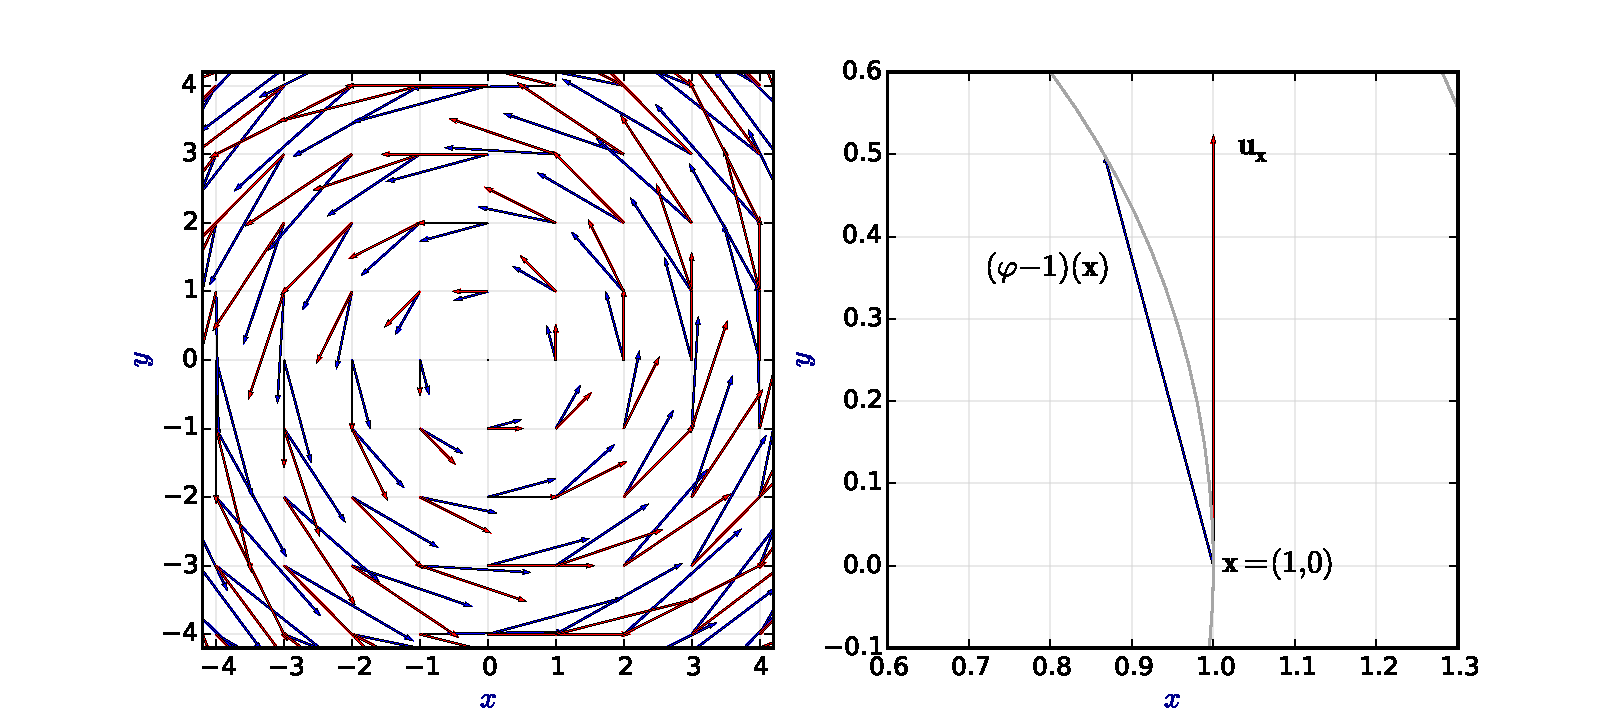
\includegraphics[scale=0.6]{figures/se2_circular_vector_field.pdf}
	\caption{the displacement field and the tangent vector field for the transformation $\varphi$ defined as a rotation of $\pi / 6$ around the origin. When $\varphi$ is subtracted by the identity function, become an element of the algebra of the velocity vector fields $\text{Vect}(\Omega)$.}
	\label{fig:se2_circular_vector_field}
\end{figure}

We define the set of \emph{deformations}, the set of continuous functions from $\Omega$ to $\Omega$, compact subset of $\mathbb{R}^d$. If a deformation is invertible with continuous inverse, then it is called \emph{homeomorphism}; the set of homeomorphisms forms a group, indicated with $\text{Hom}(\Omega)$, with the operation of function composition. If an homeomorphism is differentiable and has differentiable inverse then it is called \emph{diffeomorphism}. Again the set of diffeomorphisms forms a group, indicated with $\text{Diff}(\Omega)$.

A \emph{velocity vector field} over $\Omega$ is a differentiable function that at each point of $\Omega$, associates a vector of $\mathbb{R}^d$; the set of velocity vector fields, indicated with $\text{Vect}(\Omega)$ forms a vector space, and considering the Lie bracket defined by the directional derivative
we obtain that $\text{Vect}(\Omega)$ forms a Lie algebra\footnote{
	Some books invert the signs of the operation (see the Kirillow's remarks \cite{kirillov2008introduction} pag. 27); this choice do not have any impact in the study of the algebraic structure, but it does have an impact on the numerical results when the Lie brackets are implemented for numerical computations. At the moment the sign that defines the Lie bracket is chosen on the base of the obtained results.
}.
If $\{\frac{\partial}{\partial x_{i}}\}_{i=1}^{d}$ is a local coordinates system over $\Omega$, $\mathbf{u}=a^{i} \frac{\partial}{\partial x_{i}}$ and $\mathbf{v}=b^{i} \frac{\partial}{\partial x_{i}}$ are two elements of  $\text{Vect}(\Omega)$ written using the Einstein summation convention, the Lie bracket can be expressed using the Jacobian:
\begin{align*}
[\mathbf{u}, \mathbf{v}] &= 
a^{i} \frac{\partial}{\partial x_{i}}\big( b^{j} \frac{\partial}{\partial x_{j}} \big)
-
b^{i} \frac{\partial}{\partial x_{i}}\big( a^{j} \frac{\partial}{\partial x_{j}} \big) \\
&=
a^{i} \frac{\partial b_{j}}{\partial x_{i}}\frac{\partial}{\partial x_{j}}  
+ 
a^{i}b^{j}\frac{\partial^{2}}{\partial x_{i}x_{j}}
- 
b^{j} \frac{\partial a^{i}}{\partial x^{j}}\frac{\partial}{\partial x_{i}} 
-
b^{j}a^{i}\frac{\partial^{2}}{\partial x_{j}x_{i}} \\
&=
a^{i} \frac{\partial b_{j}}{\partial x_{i}}\frac{\partial}{\partial x_{j}}
-
b^{j} \frac{\partial a^{i}}{\partial x^{j}}\frac{\partial}{\partial x_{i}} 
= J_{\mathbf{v}}\mathbf{u} - J_{\mathbf{u}}\mathbf{v}
\end{align*}

% here the two doors
It was proved that the Lie algebra of the Lie group of diffeomorphisms $\text{Diff}(\Omega)$ is $\text{Vect}(\Omega)$ (\cite{milnor1982infinite}, \cite{ovsienko1992integrals}). 
Therefore a single vector in the Lie algebra $\text{Vect}(\Omega)$ (represented by one red arrow in figure \ref{fig:composition}) is a vector field defined over $\Omega$ (represented by the set of red arrows in figure \ref{fig:se2_circular_vector_field}). We would expect that, vice versa, to a single diffeomorphism in the Lie group corresponds a single vector of the Lie algebra. This is not the case, since Lie logarithm and Lie exponential are not local isomorphisms on the whole domain.

% % % % % % % % % % % % % % % % % % % % % % % % % % % % % % % % % % % %
% % % % % % % % % % % % % % % % % % % % % % % % % % % % % % % % % % % %
\subsection{Local isomorphisms for a subset of Diffeomorphisms: one-parameter subgroup and stationary velocity fields}\label{subse:local_isomorphisms}

In the case of matrices, the exponential map is a local isomorphisms: it is always possible to find an open neighbor of $\mathbf{0}$ in the Lie algebra and an open neighbor of the identity element in the Lie group (in the same topology induced by the metric inherited by the bigger algebra), such that the exponential map is defined and invertible.

In the infinite dimensional case there are diffeomorphisms arbitrarily close to the identity that are not embedded to any one-parameter subgroups, therefore the exponential map is not a local isomorphism (see the counterexample in \cite{milnor1984remarks}, pag. 1017 or the definition of Koppel-diffeomorphisms \cite{grabowski1988free} pag. 115).

% subset of diff in which we are interested: the one that can be parmetrized by tangent vector fields
Since for medical image registration we are interested only in the diffeomorphisms that can be parametrized by tangent vector fields, this feature is worthed to be investigated, but it requires some definitions.

% two kinds of vector fields. TVVF SVF. A continuous way to produce diffeomorphims
If $\varphi$ is a one-parameter subgroup on the manifold $\text{\emph{Diff}}(\Omega)$, then its derivative satisfies the \emph{stationary} (or homogeneous) ordinary differential equation:
\begin{align}\label{eq:generating_ODE_svf}
\frac{d\varphi(t)}{dt} = V_{\varphi(t)}
\end{align}
Where the stationary vector field $V_{\varphi(t)}$ defined over $\Omega$ is an element of the Lie algebra of $\mathcal{V}(\Omega)$ called \emph{stationary velocity field} or SVF. In fact
\begin{align*}
\frac{d\varphi(t)}{dt} 
= 
\lim_{\epsilon \rightarrow 0} \frac{\varphi(t +\epsilon)}{\epsilon} 
=
\lim_{\epsilon \rightarrow 0} \frac{\varphi(\epsilon) \varphi(t)}{\epsilon} 
=
V_{\varphi(t)}
\end{align*} 

Vice versa, given an SVF, thanks to Cauchy theorem exists always a unique solution $\varphi$ to the ODE \ref{eq:generating_ODE_svf}, given the initial condition $\varphi(0) = 1$, that satisfies the property of one-parameter subgroup.

We indicate with $\text{\emph{Diff}}^{1}(\Omega)$ the \emph{set of diffeomorphisms embedded in a one parameter subgroup}, i.e. the solutions of \ref{eq:generating_ODE_svf}. We notice that $\text{\emph{Diff}}^{1}(\Omega)$ does not form a group. In fact if $\varphi$ and $\psi$ are in $\text{\emph{Diff}}^{1}(\Omega)$ and satisfy respectively $\frac{d\varphi_1(t)}{dt} = U_{\varphi_1(t)}$ and $\frac{d\varphi_2(t)}{dt} = V_{\varphi_2(t)}$, then their composition $\varphi_1\circ\varphi_2$ does not satisfy any stationary ordinary differential equation. 
To have closure for the composition of one parameter subgroup, we have to extend our attention to non stationary (or non homogeneous) ordinary differential equation of the form:
\begin{align}\label{eq:generating_ODE_tvvf}
\frac{d\psi(t)}{dt} = W_{(t, \psi(t))}
\end{align}
Where $W_{(t, \psi(t))}$ is a non-stationary vector field, called here time varying vector field, or TVVF. If compared with to the SVF, it does not depends only on the spatial position $\mathbf{x}$ but there is also a temporal dependency. 

Think for example to a satellite orbiting around the globe: it is subject to the earth's vector field in respect to which it is constant for a fixed position, and to the lunar vector field that it is not fixed but varies in respect to the time. Conventionally the temporal domain $T$ contains the origin and formally we can write:
\begin{align*}
W : T\times \Omega & \longrightarrow  \mathbb{R}^d \\
t, \psi(t) &\longmapsto  W_{(t, \psi(t))}
\end{align*}
for $\psi$ diffeomorphism (or in the previous example, position of the satellite at time $t$) that when applied to a point of $\Omega$ is indicated with $\varphi(t,\mathbf{x})$ or $\psi^{(t)}(\mathbf{x})$.

A crucial observation for our purpose is that non-autonomous ODE are particular cases of autonomous one. Writing the diffeomorphism $\psi(t)$ applied to $\mathbf{x}$ in local coordinates as 
\begin{align*}
\psi^{(t)}(\mathbf{x}) = (\psi_1^{(t)}(\mathbf{x}), \psi_2^{(t)}(\mathbf{x}), \dots ,\psi_d^{(t)}(\mathbf{x})) \in \mathbb{R}^{d}
\end{align*}
Defining a new function $\psi_0^{(t)}(\mathbf{x}) = t_0 + t$ for all $\mathbf{x} \in \Omega$, we can obtain then the new diffeomorphism $\tilde{\psi}^{(t)}$ that in local coordinates is expressed as 
\begin{align*}
\tilde{\psi}^{(t)}(\mathbf{x}) = (\psi_0^{(t)}(\mathbf{x}), \psi_1^{(t)}(\mathbf{x}), \psi_2^{(t)}(\mathbf{x}), \dots ,\psi_d^{(t)}(\mathbf{x})) \in T\times \mathbb{R}^{d}
\end{align*}
that reduces the ODE \ref{eq:generating_ODE_tvvf} to an ODE of the form \ref{eq:generating_ODE_svf}. In the example of satellite, is like considering the temporal dimension as an additional dimension of the space. The vector that influence the satellite is an SVF for every point in the domain of space-time. 

It follows that tationary ODE and non-stationary ODE have solutions that belong to $\text{\emph{Diff}}^{1}(\Omega)$ and $\text{\emph{Diff}}^{1}(T\times \Omega)$ respectively. For each instant of time the solution of non-stationary ODE, are embedded in the set of one-parameter subgroup of $\text{\emph{Diff}}(\Omega)$, but for two different instant of time, the solution can belongs to two different elements in the one parameter subgroups. 

In conclusion, we have that there in the case of diffeomorphisms $\exp$ is not a local isomorphism, unless we do not restrict the group of diffeomorphisms to the one embedded in a one parameter subgroup $\text{\emph{Diff}}^{1}(T\times \Omega)$. In addition the set of diffeomoerphisms restricted to the one that solves the equation \ref{eq:generating_ODE_svf} does not form any group with the composition. This happen only if we extend to the solution of the non stationary ODE \ref{eq:generating_ODE_tvvf}, and therefore to TVVF. In addition, indicating with $\text{SVF}$ the set of stationary velocity fields and with $\text{TVVF}$ the set of time varying velocity fields, we have that
\begin{align*}
\text{\emph{Diff}}^{1}(\Omega) &= \exp(\text{SVF}) = \exp(\text{TVVF})
\end{align*}
but to a given SVF exists only one one-parameter subgroup $\varphi$ that satisfies the ODE \ref{eq:generating_ODE_svf}. The same thing does not necessarily happens for the TVVF.

In the LDDMM framework \cite{beg2005computing} TVVFs are initially considered, while with the paper of Arsigny \cite{arsigny2006log}, and in subsequent works, the attention has been restricted to SVF, in order to be able to use the scaling and squaring and the inverse scaling and squaring algorithms for the numerical computation of the Lie exponential and the Lie logarithm. In fact the scaling and squaring method, as every numerical method based on the phase flow \cite{ying2006phase}, works only under the assumption that the transformation belongs to the same one-parameter subgroup.


% % % % % % % % % % % % % % % % % % % % % % % % % % % % % % % % % % % %
% % % % % % % % % % % % % % % % % % % % % % % % % % % % % % % % % % % %
\subsection{A bigger algebra for the group of Diffeomorphisms}\label{subse:bigger_algebra}
As well as for any matrix Lie group, both the group $SE(2)$ and the algebra $\mathfrak{se}(2)$ are subset of the same bigger algebra of matrices in the general linear group $GL(3,\mathbb{R})$. The product of the algebra coincides with the composition of the group and thanks to the linearity, scalar product is compatible both with the product and the composition.

The existence of a bigger algebra is not important only in the research of an elegant structure: the power series expansions of the exponential (\ref{eq:exp_as_inf_sum}) and the logarithm (\ref{eq:log_as_inf_sum}) as well as expressions like (\ref{eq:prop_matrix_diff_log}) and (\ref{eq:prop_matrix_lim}) would be meaningless without the possibility of expressing the sum of two elements of a multiplicative group. Moreover, if the bigger algebra that contains both Lie group and Lie algebra exists, a unique norm in this space can be defined and utilized to compare elements in the both subspaces.

In the case of diffeomorphism of the compact subset $\Omega$ of $\mathbb{R}^d$, we can identify a bigger vector space that contains both Lie group and Lie algebra, but it is less straightforward than in the case of matrices, and for this aim it is necessarily to have some definitions at hand.

\begin{figure}[!ht]
	\centering
	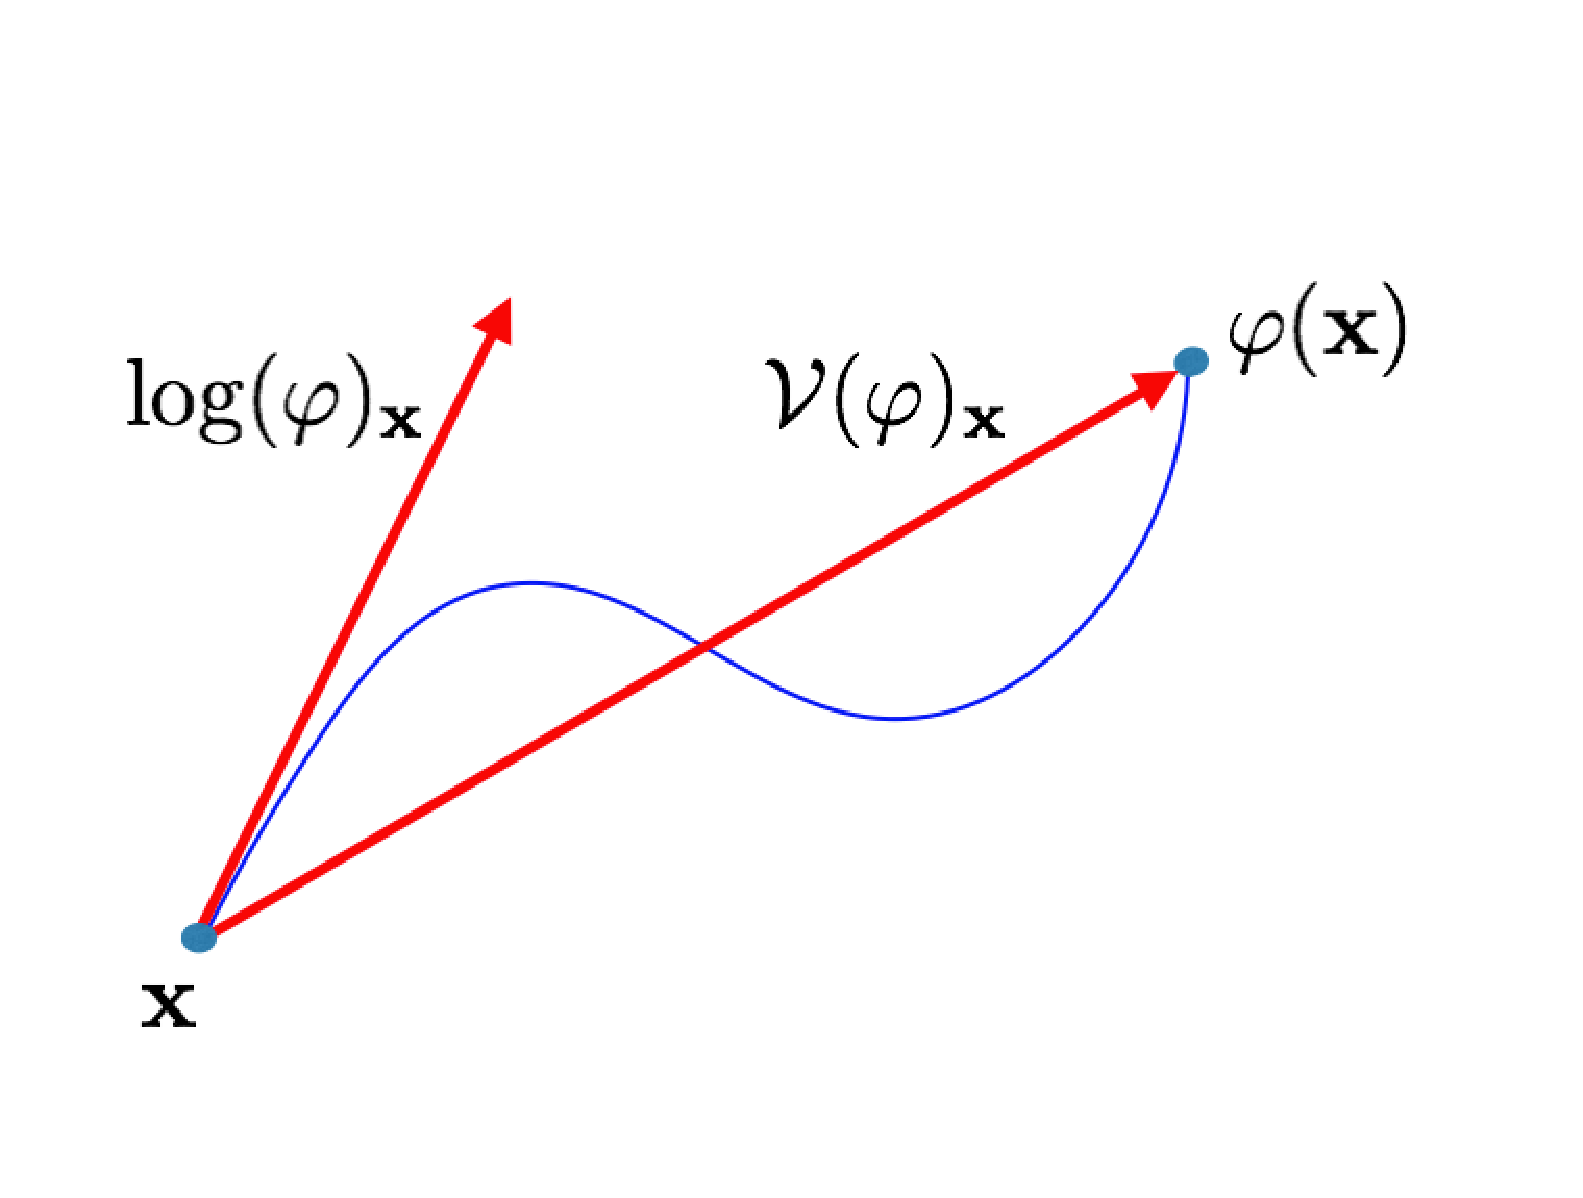
\includegraphics[scale=0.25]{figures/exp_versus_v.pdf}
	\caption{for small deformations, the displacement field $\log(\varphi)$ and the tangent field $\mathcal{V}(\varphi)$, computed at the point $\mathbf{x}$ of $\Omega$, are close to each others.}
	\label{fig:exp_versus_v}
\end{figure}

There are two ways to associate a diffeomorphisms $\varphi$ to a velocity vector field. The first one is elementary but fundamental in this context: it consists in subtracting to $\varphi$ the identity function $1$. If $\mathbf{x}$ is in $\Omega$ and $\varphi(\mathbf{x})$ is the new point after the transformation, then the associated velocity vector field, called here \emph{displacement field of} $\varphi$, is the function that at the point $\mathbf{x}$ associate the vector defined as the difference $\varphi(\mathbf{x}) - \mathbf{x}$. To recover the deformation from a velocity field $\mathbf{u}$ is enough to add the identity; in this case we have the \emph{deformation of} $\mathbf{u}$. We indicate this operation of adding and subtracting the identity with the function $\mathcal{V}$:
\begin{align*}
\mathcal{V}(\varphi) = \varphi - 1 
\qquad \qquad
\mathcal{V}^{-1}(\mathbf{u}) = \mathbf{u} + 1 
\end{align*}
We can see that displacement fields of diffeomorphisms are elements of $\mathcal{V}(\Omega)$, that is the analogous of the bigger algebra that contains Lie group and Lie algebra in the case of matrices. We can observe that this operation of subtracting the identity to the deformation has already been used implicitly in the power series expansion of the Lie logarithm for matrices, see equation \ref{eq:log_as_inf_sum}.

The second way to associate a velocity vector field to $\varphi$ is with the Lie logarithm defined in the chapter \ref{ch:tools}. It is interesting to notice that when $\mathbf{u}$ is small then $\mathcal{V}^{-1}$ and $\exp$ are closed to each other and $\mathcal{V}^{-1}$ can be considered a good approximation of $\exp$ (see figure \ref{fig:exp_versus_v}). The very same happens for matrices, as noticed in equations (\ref{eq:small_rotation_matrices_approx}).

At this point it is important to notice that, while a displacement field of $\varphi$ can always be defined, the exponential map it is not defined for any diffeomorphism. This is the second remarkably difference between the matrix Lie group and the Lie group of diffeomorphisms that will be investigated in the next section.



% % % % % % % % % % % % % % % % % %
% % % % % % % % % % % % % % % % % % %
\subsection{A Norm for the Elements in the one-parameter subgroup}\label{subse:norm}
A metric between tangent vector fields of $\Omega$ can be defined as 
\begin{align}\label{def:metric_two_svf}
d(\mathbf{u}, \mathbf{v}) 
= 
\Big( \int_{\Omega} \euclideanMetric{\mathbf{u} - \mathbf{v}}_{L^2}^{2} d\mathbf{x} \Big)^{1/2}
\end{align} 
that naturally induces a metric on the Lie algebra.

The Lie group $\text{\emph{Diff}}^{1}(\Omega)$ do not possess any norm, but the corresponding displacement fields defined by $\mathcal{V}$, as tangent vector fields does. Given two diffeomorphisms $\varphi_0$ and $\varphi_1$ we have
\begin{align}\label{def:metric_two_displacement_field}
d^{1}(\varphi_0,\varphi_1) 
= 
\Big( \int_{\Omega} \euclideanMetric{\mathcal{V}(\varphi_0) - \mathcal{V}(\varphi_1)}_{L^2}^{2} d\mathbf{x} \Big)^{1/2}
\end{align} 
Despite the limitation that Lie algebra and Lie group of diffeomorphisms are not subset of the same bigger algebra, we can nevertheless consider a function that measure the best approximation of metric we can have for $\text{\emph{Diff}}^{1}(\Omega)$ and SVF:
\begin{align}\label{def:metric_one_svf_one_displacement_field}
d^{m}(\mathbf{u},\varphi) 
= 
\Big(\int_{\Omega} \euclideanMetric{\mathbf{u} - \mathcal{V}(\varphi)}_{L^2}^{2} d\mathbf{x} \Big)^{1/2}
\end{align} 
The next section is about the parametrization of SVF in the applications, and it is followed by the one that presents the numerical methods for the log-composition when applied to SVF.

% % % % % % % % % % % % % % % % % %
% % % % % % % % % % % % % % % % % % %
\subsection{Parametrization of SVF: Grids and Discretized Vector Fields}\label{se:parametrization_SVF}

Even if images are discrete elements, the underpinning model of the transformations is based on the continuous. There are several motivations that led to this choice: as underlined by \cite{szeliski1994image}, the most important is that images are discrete measurement of the continuous property of an object. Therefore it is reasonable have a model as close as possible to the continuous object rather than to a set of discrete measurements. 
Certainly it is important to keep in mind the fact that the continuous approximation is obtained - in a non unique way - from the discretized image with an interpolation scheme. This imply that, for example if the distance between two separate objects is less than the size of a voxel, in continuous approximation based on the discretized image the two object will be not anymore separated. 

Also transformations between images are discretized vector fields, where each vector is applied to an element of a grid. These transformations can only be considered as a model of the group of diffeomorphisms (a model of a model, in image registration!) and reflects only partially the continuous property of the original transformation.
On the other side the possibility of working with discretized elements means working with something that can be managed by computers.

As in many implementation, the data structure utilized to store images, as well as displacement fields are 5-dimensional matrices
\begin{align}\label{eq:basic_data_structure}
M = M(x_i,y_j,z_k,t,d) \qquad (i,j,k)\in L , ~~ t \in T  ~~ d = 1,2,3
\end{align}
where $(x_i,y_j,z_k)$ are discrete position of a lattice $L$ in the domain of the images, $t$ is the time parameter in a discretized domain $T$ and $d$ is index of the coordinate axis. So, the discretized \emph{tangent vector} $\mathbf{v}_{\tau}(x_i,y_j,z_k)$ at time $t$, has coordinates defined by
\begin{align*}
\mathbf{v}_{t}(x_i,y_j,z_k) = (M(x_i,y_j,z_k,t ,1), M(x_i,y_j,z_k,t,2), M(x_i,y_j,z_k,t ,3))
\end{align*}


% % % % % % % % % % % % % % % % % %
% % % % % % % % % % % % % % % % % % %
\subsection{Computations of Log-composition for SVF}\label{se:log_composition_SVF}
A closed-form for the Taylor Expansion method \ref{se:taylor_expansion} to compute the log-composition with elements in $\text{\emph{Diff}}^{1}(\Omega)$ is not known. We will therefore compare the truncated BCH formula with the parallel transport method \ref{se:parallel_transport}. 
The Lie bracket that appears of SVF in the truncated $BCH$ of degree $0,1,1.5$ and $2$, are computed using the Jacobian matrix $J$:
\begin{align}
[\mathbf{u},\mathbf{v}] :=J_{u}\mathbf{v} - J_{u}\mathbf{v}  
\qquad
\forall \mathbf{u},\mathbf{v} \in \mathfrak{g}
\end{align}
as a consequence of its definition (see \cite{lee2012introduction}).
It has been shown that this definition is uniquely defined as action on the space of $\mathbb{C}^{\infty}$ function on the same domain and it satisfies the axioms of Lie bracket of a Lie algebra.\\

Therefore the truncated approximation of the BCH formula presented in the equation \ref{eq:bch_definition} become:
\begin{align*}
BCH^{0}(\mathbf{u},\mathbf{v}) &= \mathbf{u} + \mathbf{v} \\
BCH^{1}(\mathbf{u},\mathbf{v}) &=  \mathbf{u} + \mathbf{v} + \frac{1}{2}(J_{\mathbf{u}}\mathbf{v} - J_{\mathbf{u}}\mathbf{v})\\
BCH^{3/2}(\mathbf{u},\mathbf{v}) 
&=  
\mathbf{u} + \mathbf{v} + \frac{1}{2}(J_{u}\mathbf{v} - J_{u}\mathbf{v}) + 
\frac{1}{12}\big( 
2 J_{\mathbf{u}} J_{\mathbf{u}}\mathbf{v} +2 J_{\mathbf{u}} J_{\mathbf{v}}\mathbf{u}
- 
J_{(J_{\mathbf{u}}\mathbf{v} - J_{\mathbf{u}}\mathbf{v})}\mathbf{u} 
\big) 
\\
BCH^{2}(\mathbf{u},\mathbf{v}) 
&=  
\mathbf{u} + \mathbf{v} + \frac{1}{2}(J_{u}\mathbf{v} - J_{u}\mathbf{v}) 
\\
&+ 
\frac{1}{12}\big( 
2 J_{\mathbf{u}} J_{\mathbf{u}}\mathbf{v} +2 J_{\mathbf{u}} J_{\mathbf{v}}\mathbf{u}
- 
J_{(J_{\mathbf{u}}\mathbf{v} - J_{\mathbf{u}}\mathbf{v})}\mathbf{u} 
+
2 J_{\mathbf{v}} J_{\mathbf{v}}\mathbf{u} +2 J_{\mathbf{v}} J_{\mathbf{u}}\mathbf{v}
- 
J_{(J_{\mathbf{v}}\mathbf{u} - J_{\mathbf{v}}\mathbf{u})}\mathbf{v} 
\big) 
\end{align*}
Lie brackets of SVF can become extremely small, in particular, as we will see in the last chapter, when the standard deviation of the Gaussian filter that generates the fields is small. \\
Whether it is not known how to apply Taylor method presented in \ref{se:taylor_expansion} for the SVF, the parallel transport method for the computation of the log-composition follows directly from equation  \ref{eq:parallel_transport}:
\begin{align*}
\mathbf{u}_0\oplus \mathbf{u}_1
&\simeq
\mathbf{u}_0 
+
\exp_{e}\big(\frac{\mathbf{u}_0}{2}\big)   
\circ  \exp_{e}(\mathbf{u}_1) 
\circ \exp_{e}\big(-\frac{\mathbf{u}_0}{2}\big)
-
e
\end{align*}
Here the exponential function can be computed with several algorithms (scaling and squaring, forward Euler, composition method, Taylor expansion, see \cite{bossa2008algorithms} for a comparison of their performances). Following the original setting of the Log-euclidean metric proposed in \cite{arsigny2006log} we use the scaling and squaring, keeping in mind that this choice impact on the results.








